\subsection*{Syringe Pump construction}
The presented syringe pump system is composed of a mechanical assembly, an electronic controller board, and an accompanying firmware/software stack that affords different levels of control over the system's behavior. 
All resources (interface software, firmware, and mechanical designs) are available from \url{https://github.com/harp-tech/device.syringepump}.

\subsubsection*{Mechanical construction}
The mechanical assembly of the syringe pump was designed to be easily produced and assembled without any particular expertise. All parts necessary for the build are included in the bill of materials. Most parts are readily available off the shelf. Additionally, custom structure parts can be in-house laser-cut and 3D printed, if such resources are available, or sourced from third-party manufacturers, using the provided designs. In addition to the bill of materials, we also documented the assembly process with step-by-step instructions, including photographs, that should be followed to guarantee the best possible assembly of the structure.

In the provided mechanical configuration, we opted for a NEMA 17 Stepper motor (HT17-275 from Applied Motion) due to its high precision and torque rating. Specifically, the combination of motor step resolution (1.8 $\deg$/step) together with a 0.8 mm pitch length driving rod leads to a theoretical linear resolution of 4 $\mu m$/step, which can be further increased by using step multipliers of up to 1/16.
Additionally, to characterize the system, we chose two glass syringes models with total volumes compatible with those routinely used for animal experiments (5 and 10 $mL$, 1000 Series Syringes, Hamilton). Taking their cross-section diameter into consideration, the final single-full-step theoretical resolution will be 0.33 and 0.66 $\mu L / step$ for the 5 and 10 $mL$ syringe models, respectively.

It should be noted, however, that the present system will be able to accommodate a large range of other options (be it stepper motors or syringes), with little to no modifications to the suggested design.

\subsubsection*{Electronics}

The syringe pump is controlled by a custom-made printed circuit board which is comprised of three main blocks: a microprocessor, an interface logic circuitry and, a motor driver \cref{fig:PumpDrawing}.

The microprocessor block consists of an ATxmega microprocessor (ATXMEGA128A4U-AU, Microchip Technology) that implements the Harp protocol \url{https://github.com/harp-tech/protocol}, a USB to serial UART interface and a stereo phone jack for temporal synchronization between Harp devices. The Harp protocol allows the syringe pump to be flexibly controlled externally through the USB interface with any host implementing the Harp API (\textit{e.g.:} via Bonsai\citep{Lopes2015} or Python).

The interface circuitry block consists of logic buffers that provide a direct low-level interface with the micro-stepper driver (A4988SETTR-T, Allegro Microsystems) to the user (bypassing the microcontroller block). Moreover, it provides access to the I/O breakout that can be used to trigger protocol delivery with other external, TTL-compatible, devices, supporting input voltages up to 5V. The voltage of the digital outputs can also be configured in the board through a jumper to select between 3.3V and 5V voltage output logic.

The modularity of the board design affords users the option to assemble a simpler version without the microcontroller block, for applications wherein low-level control is sufficient. This significantly cheaper version is assembled using the same PCB schematic, with minimal changes to the board components, and can be found in an alternative bill of materials provided.

Despite having been designed for the herein described configuration, the design of the control system (including the Harp API) is compatible with other types of bipolar stepper motors (assuming an output drive capacity of up to 12V and ±1.7A).

\subsubsection*{Syringe pump user control}

We designed the syringe pump system to with three distinct interface levels, that afford experimenters control over the pump according to their experimental needs. In addition to \cref{fig:PumpControl}, we offer a brief description of the three available options:
\begin{itemize}

\item{Low-level control} - This option relies on directly controlling the I/O interface of the micro-stepper driver. This is achieved by using an external source (\textit{e.g.:} Arduino microcontroller) to generate the necessary input logic. Eight inputs lines are exposed: GND (ground), EN (enables the driver when low), MS1-3 (determines the step-size of the motor, 1 to 1/16 times a full step), DIR (determines the direction of rotation) and STEP (triggers a micro-step). It should be noted that this control logic is common and documentation is extensively available.
Additionally, the PCB exposes two outputs that correspond to "end-of-travel" switches, that can be used to implement operation safety-stops.
This control option does not require the full board to be assembled, as it does not rely on the microcontroller block for control and, while it affords the user the most flexibility, it requires an external source of logic control that might be cumbersome to set up and unnecessary for the vast majority of applications. Thus, the next two options abstract some of the low-level control away from the user at the cost of some flexibility.

\item{Trigger-based Control} - This option allows the user to configure a \textit{“protocol”} that is triggered with the detection of a TTL rising edge. This control logic is extensively used across many platforms (\textit{e.g.} Med associates, Open-Ephys, Arduino) making the system easily integrated with existing experimental rigs.
The protocol can be configured via a custom-designed graphic user interface \ref{fig:PumpControl} that leverages the Harp protocol to configure the microcontroller. Available settings currently include an option to run in “Step Mode”, wherein the user sets number, duration, and frequency of the steps per protocol). The behaviour of the I/O pins can be configured via this GUI to provide users with hardware events that can be used to interface with third-party devices (e.g. see \ref{fig:Ephys})
It should be noted that, contrary to the previous mode, “end-of-travel” events (\textit{i.e.,} when the limit switches are triggered) are automatically handled by the controller, to prevent accidental mechanical damage to the system.

\item{Software Control} - The third option allows the user to control the syringe pump system through a software API. This option can be seen as an extension of the last, with the protocol being triggered by a software, instead of an hardware event. This option is available to any host running the Harp API, namely Bonsai. Bonsai is a visual programming language that specializes in asynchronous data acquisition and has seen growing adoption from the neuroscience community. Users can change an large number of settings (identical to the “triggered control” version) and trigger a protocol on any Bonsai event. As an example, the user can periodically deliver a constant amount of reward \ref{fig:PumpControl}, dynamically change the amount of liquid delivered on every trial, contingent on some behaviour/physiological event, or trigger the delivery of water aligned to when the animal enters a given area of an arena.
Finally, the Harp protocol allows the user access to hardware timestamped events (\textit{e.g.} protocol onset), allowing for easy event alignment.

\begin{figure*}
	\centering
	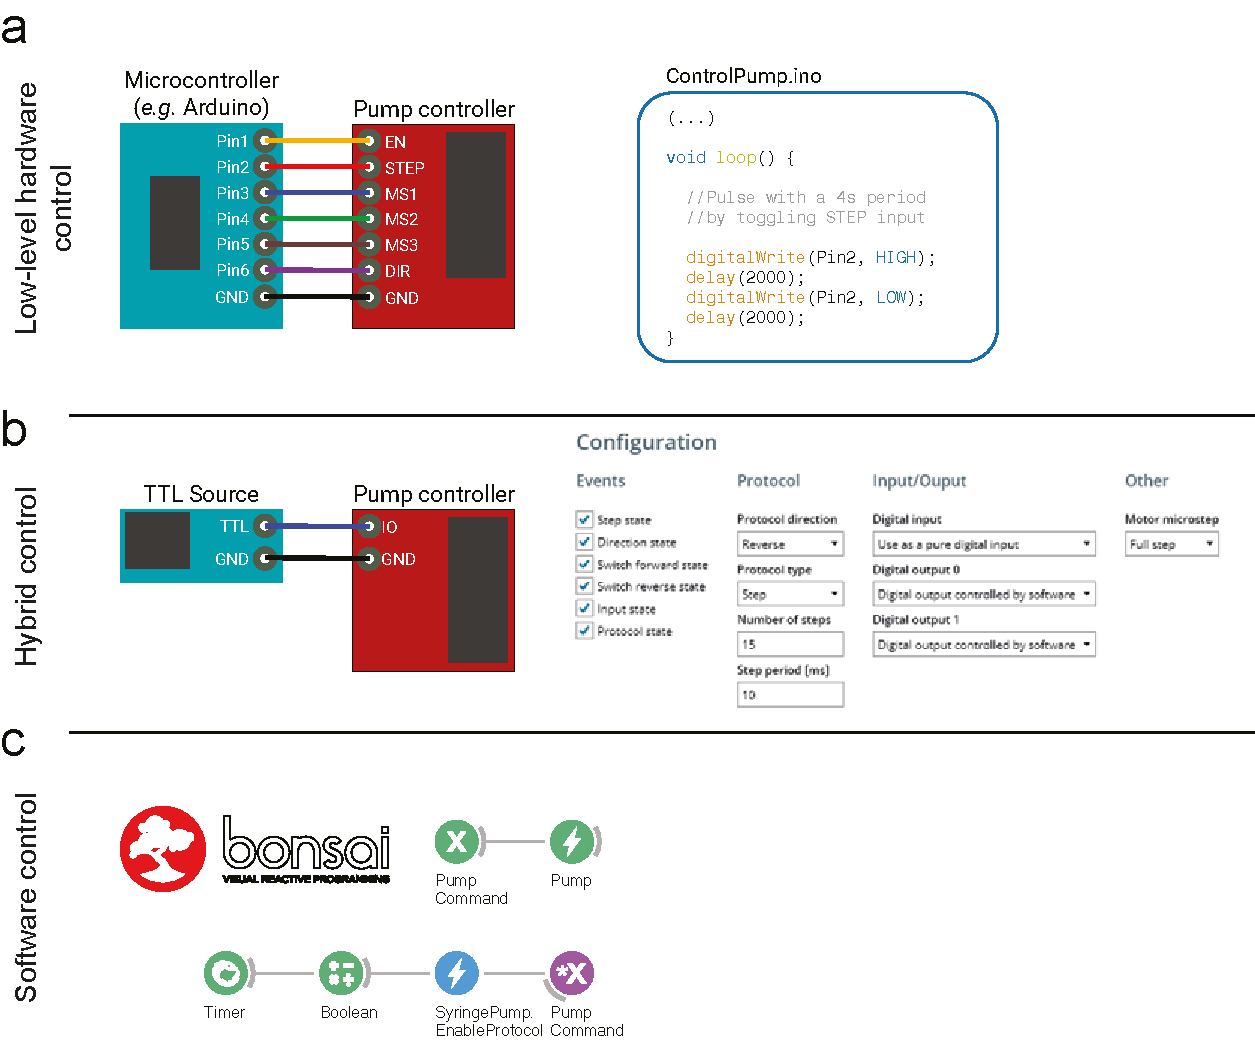
\includegraphics[width=1.0\linewidth]{Figures/Artboard 4.pdf}
	\caption{\textbf{The current system affords three distinct levels of interface.}\\
		(\textbf{a}) Low-level hardware control expects the user to fully define the control logic for the stepper motor driver. This can be achieved by implementing such logic in a microcontroller (\textit{e.g.} Arduino, right textbox) that defines the state of all input control pins to the stepper-motor driver. It should be noted that this mode does not require the full PCB to be populated, since it does not rely on the Harp core protocol implementation. \textbf{b}) Trigger-based control allows the user to use an external trigger event (via transistor-transistor logic, TTL) to playback a pre-defined delivery protocol. The default protocol values (\textit{e.g.} volume and flow-rate) can be modified using a provided graphical-user interface, or Bonsai. \textbf{c}) Software control allows the user to fully parameterize, and trigger, protocols from a computer host running Bonsai without the need for any external hardware triggers. Sub-millisecond synchronization can be achieved via Harp protocol, or by an configurable digital output event.}
	\label{fig:PumpControl} 
\end{figure*}

\end{itemize}

\subsection*{Calibration}
\subsubsection*{Large volume calibration}
The pump is compatible with a wide variety of syringes. However, it is advisable to calibrate the full system to account for potentially significant differences across parts. Small volumes of delivered liquid are technically challenging to measure, as a result, calibrating liquid delivery systems is usually performed by repeating the same protocol a large number of times. This strategy rests on the assumption that single steps are relatively reproducible and the mean across several dozens to hundreds of repetitions is thus representative. We calibrated the system by varying the number of steps per protocol, which was then repeated 200 times, waiting 250 ms between the end of each protocol and the start of the next. We then weighted the amount of collected liquid to yield the total collected volume (we assumed a water density of 1g/mL at room temperature). Single protocol volume was thus given by \ref{eq:LargeVolumeCalibration}:

\begin{equation} \label{eq:LargeVolumeCalibration}
    V_{single}(mL) = \frac{Weight (g)}{1 (g/mL)} * \frac{1}{200}
    \end{equation}

To assess reproducibility across runs, we repeated this protocol twenty times. Depending on the experiment, we also adjusted the range of calibration values. Critically, all tested volumes laid on top of a linear calibration regime, and outcomes were consistent with the predicted theoretical volumes \cref{eq:LargeVolumeCalibration}.

We followed protocol identical to the syringe pump system to calibrate the solenoid valves (LHDA1231215H, Lee Co.). Briefly, we calibrated the valves by setting the water reservoir (a 20mL plastic syringe) at a height identical to what we routinely use in our laboratory for behavioural experiments ($\sim$30cm). We systematically varied the opening time (between 10 and 150 ms) to yield different delivered volumes. Both the number and time between trials were identical to the ones used in the pump systems. Hardware control logic was implemented in an Arduino Microcontroller (Arduino Mega, Arduino).

\subsubsection*{Single bolus calibration}

While technically amenable, measuring the outcome of several hundred protocols might obscure variability across single trial events. We thus developed a simple computer-vision-based method to measure small volumes. Briefly, the end of a syringe was fitted with a plastic adapter with a small glass capillary (Model 211713, Vitrex) glued to the end (\cref{fig:PumpDrawing}). A computer vision camera (Model FL3-U3-13S2C-CS, FLIR) was used to image the capillary.
In order to increase the contrast between liquid and background, we diluted a small amount of red colourant (Erythrosin B, Sigma-Aldrich) that, when combined with LED illumination, resulted in the image shown in \cref{fig:PumpProtocol}.

The video acquisition and processing routine were implemented in Bonsai. To measure the amount of displaced liquid inside the capillary, we defined a region of interest, excluding optical artifacts resulting from glass-induced diffraction, and binarized the image thresholding the pixel values in RGB colour space. We then used this binarized image to segment the area corresponding to the displaced liquid volume. We choose the horizontal axis of the region as our reported metric. Data were acquired at 10 frames-per-second and synchronization was achieved by sending a short TTL pulse to the camera each time a protocol was started. Syringe pump control logic was implemented using the low-level control mode of the system and an Arduino microcontroller.

Unless otherwise stated, the inter-pulse-interval was set to 4 milliseconds. Before each run, up to 5 small pulses were applied to ensure that every protocol started from comparable conditions. These pulses were discarded from all analyses. The interval between each protocol was drawn from a uniform distribution (10 to 20 s). Due to the size of the capillary, some volume values required cleaning the tube between trials. We cleaned it by flushing ethanol and air-drying it.

For the dynamic flow rate experiment shown in \cref{fig:FlowRateControl}, the inter-pulse-interval was systematically varied in order to control the output flow rate. We estimate flow rate by linearly fitting, on each trial, the displaced area to time (between protocol onset and the stabilized epoch).

\subsection*{Experimental validation}

\subsubsection*{Animal behaviour experiments}
Two Long Evans, 5 month-old, male rats were trained on a variant of a Two-armed bandits task \citep{Ito2009} to assess reward preference. Briefly, subjects were placed in an experimental box with access to four nose ports, two for initiation, and two for reward delivery. Reward volumes were drawn from a pre-defined set of calibrated values (3.46, 6.92, 13.84, 27.68, and 55.36 $\mu$L) and delivered using the syringe pump system. A light on top of the initiation ports signalled trial availability. After initiating, animals were required to fixate at the centre nose port for a short period of 100 milliseconds, after which they would be allowed to collect a reward at one of the two side-reward ports. Importantly, the amount of water delivered at any port was constant within a given session block, but always different across the two ports. After reaching a preference criteria of >80\% towards the highest reward nose-port over the last 15 trials, a block transition would be triggered, the trial initiation switched to the opposite nose port (\textit{e.g.:} odd and even numbered blocks would be initiated at the north and south nose ports, respectively). At block transitions, we forced reward amounts on each nose-port to be different, but otherwise allowed for any other combination. In particular, the highest rewarded nose-port need not to change between blocks.


\subsubsection*{Compatibility with electrophysiological recordings}

Previous studies report induced electrical artifacts from some syringe pump systems \citep{Amarante2019}. We thus tested the compatibility of our system with electrophysiological techniques by recording these signals while triggering the micro-stepper driver in close proximity.
We followed the protocol for acute recordings previously described in \cite{Cruz2022}. In short, mice (8-10 weeks old) were anaesthetized with Isoflurane (1-2 \% at 0.8L/min) and a small straight metallic head-post was securely cemented to the skull. Animals were given a dose of Carprofen on the day of the surgery, and were allowed to recover for a minimum of 5 days. Prior to the recording session, a small circular craniotomy (1.5mm of diameter) was opened above the dorsal striatum. During acquisition, animals were head-restrained by a custom-made apparatus and allowed to run on top of a rotatable cylinder. A silicon probe (ASSY 77-H2, Cambridge NeuroTech) was slowly lowered (2-10$\mu$m/s) into the dorsal striatum ($\sim$3mm from brain surface). We allowed a minimum of 30 minutes before recordings began. Headstage data was digitized at 30kHz and acquired using the Open-Ephys Acquisition board and Bonsai. In order to align electrophysiology data with pump events, we used the aforementioned “Triggered Control” mode and configured one of the controller’s outputs to report STEP events via TTL, which was then acquired with the same Open-Ephys acquisition board. The syringe pump was positioned ~20cm away from the animal without any electromagnetic shielding material in-between. Protocols were manually triggered by the experimenter.
Electrophysiological data shown in \cref{fig:Ephys} was minimally processed by applying a Butterworth digital bandpass filter (0.3 to 8kHz).

\subsection{Code and data availability}
All code and data related to the device characterization shown in this manuscript are available from \url{https://github.com/fchampalimaud/syringe.pump.manuscript}.


